%Template file for MATH96012 project 3 discussion and figures
\documentclass{article}
\usepackage{placeins}
\usepackage[utf8]{inputenc}
\title{MATH96012 Project 3}

\author{\emph{Alexander John Pinches CID:01201653}}

\usepackage{graphicx}

\begin{document}

\maketitle



%---------------- Question 2 -------------------
\section*{Question 2}
We compare the different implimentations for different M,N and Nt values.
We would expect as Nt increases a linear increase in time taken this is shown
in figure \ref{figNt} with fortran implimentations being faster as they can optimise over the for loop unlike a interpreted language. OMP+F90 the fastest but as we increase Nt they all increase linearly with Nt.
 We see for large N and M in figures \ref{figN} and 
\ref{figM} that the OpenMP implimentation offers a speed up over
fortran and python except for large N. The speed up of the parallelisation is greater with increasing M than increasing N. The increase suggests the code is very
parallelisable though as the differences between the F90+OMP implimentation and the F90 implimentation is large.
This is as most of the parallel loops are over M not N. The slowdown of fortran implimentations vs the python implimentation is likely caused by 
fortran using column-major array storage and C using row-major changing the positions of each element in memory. We would ideally like to average these to check but that would take too long. So for very large M and/or Nt we should use the fortran+OMP implimentation for large N python is faster. To find the
exact point we should switch over we could do a grid search of values but this would take a very long time. 





\subsection*{Figures}
\begin{figure}[h!]
\centering
%Uncomment line below to display figure saved as fig31.png
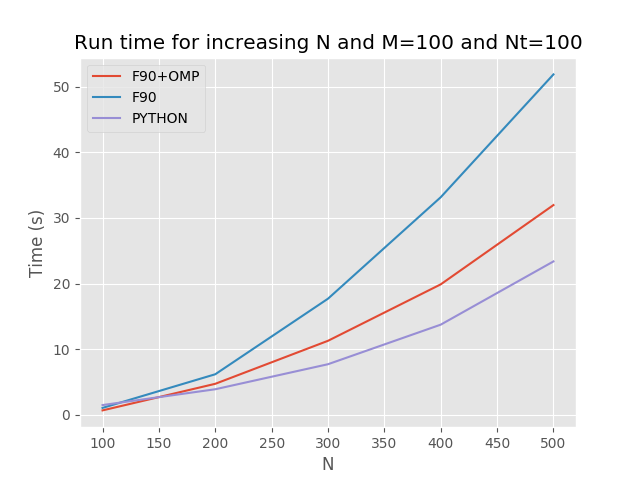
\includegraphics[width=0.6\textwidth]{n_time_comparison.png}
\caption{Time to run for varying N}
\label{figN}
\end{figure}
\FloatBarrier
%Add further figures as needed here
\begin{figure}[h!]
\centering
%Uncomment line below to display figure saved as fig31.png
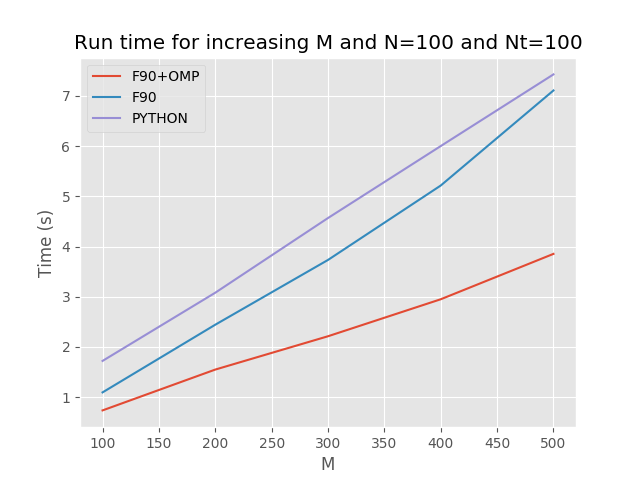
\includegraphics[width=0.6\textwidth]{m_time_comparison.png}
\caption{Time to run for varying M}
\label{figM}
\end{figure}
\FloatBarrier
\begin{figure}[h!]
\centering
%Uncomment line below to display figure saved as fig31.png
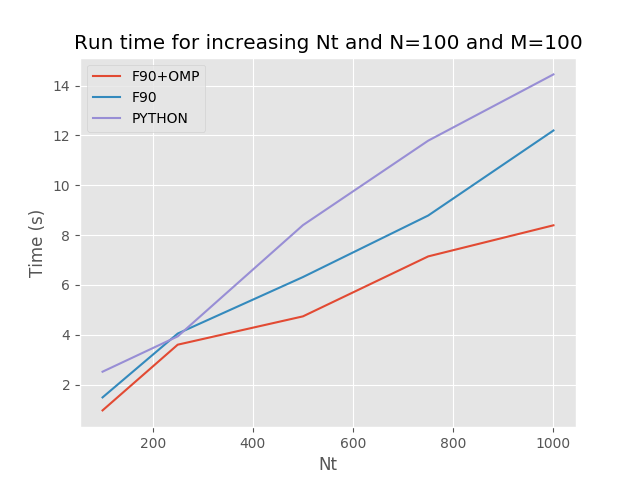
\includegraphics[width=0.6\textwidth]{nt_time_comparison.png}
\caption{Time to run for varying Nt}
\label{figNt}
\end{figure}
\FloatBarrier

%Add further figures as needed here

%---------------- End Question 2 -------------------


%---------------- Question 3 -------------------

\section*{Question 3}
We see that as $\tau$ increases the correlation decreases. We expect this
as although random they interact with one another making them correlated for small lags
but as they disperse they will interact less with each other making their positions less correlated. This shows that particles tend to disperse over time.
The correlation overall is very low though this is due to the large random element caused by A.

Increasing M will just make the function more smooth as alpha is averaged over M. 

\subsection*{Figures}


\begin{figure}[h!]
\centering
%Uncomment line below to display figure saved as fig31.png
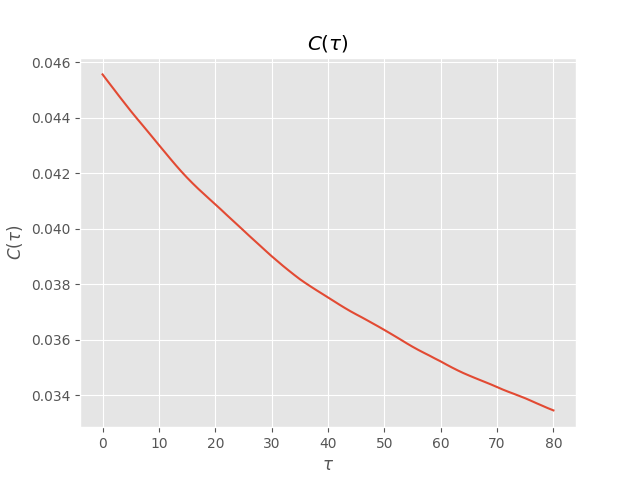
\includegraphics[width=0.6\textwidth]{corr.png}
\caption{Correlation for lag $\tau$}
\label{figCorr}
\end{figure}
%---------------- End Question 3 -------------------






%---------------- End document -------------------


\end{document}
